% !TeX program = lualatex
% !TeX encoding = UTF-8

\documentclass[x11names, border=5pt]{standalone}

\usepackage{tikz}
\usetikzlibrary{decorations.pathmorphing}
\usetikzlibrary{decorations.markings}
\usetikzlibrary{arrows.meta,bending}

\begin{document}
	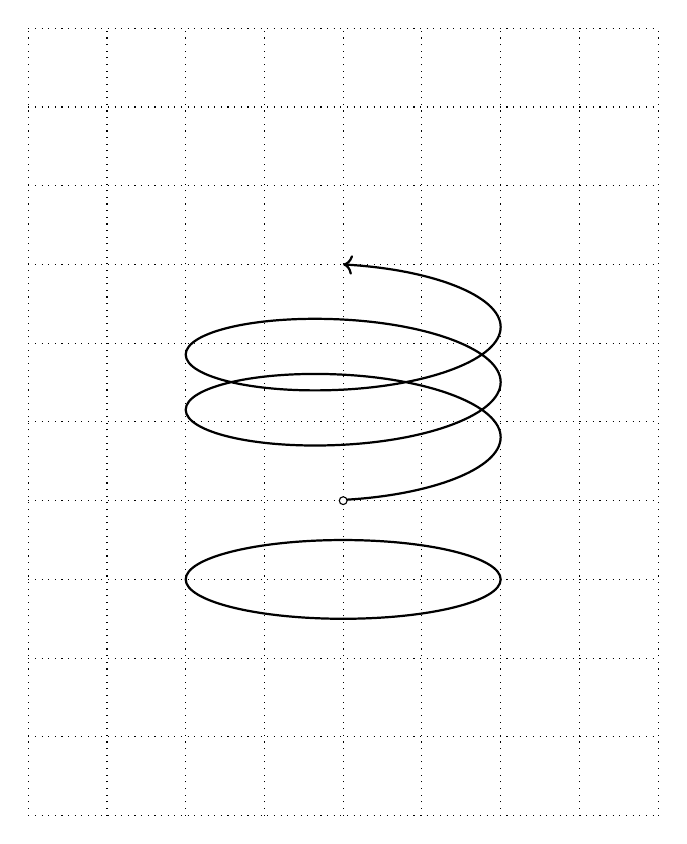
\begin{tikzpicture}
		\draw[dotted] (-4,-3) grid (4,7);
		\draw[thick] (0,0) ellipse (2cm and 0.5cm);
		\draw[thick,decoration={aspect=0.31, segment length=7mm,
					amplitude=2cm,coil},decorate,arrows = {<[bend]-}] (0,4) --(0,1);
		\node[draw,fill=white,circle,inner sep=1pt] at (0,1){};
	\end{tikzpicture}
\end{document}
